\documentclass{article}
\usepackage{amsmath}
\usepackage{amsfonts}
\usepackage{graphicx}
\usepackage[usenames, dvipsnames]{color}
\usepackage{multirow}
\usepackage{tabularx, booktabs}
\usepackage{longtable}
\usepackage{caption}
\usepackage{colortbl}
\usepackage{url}
\usepackage{hyperref}
\usepackage{wrapfig}
\usepackage{listings}

\usepackage[top=1in, bottom=1in, left=1in, right=1in]{geometry}

\definecolor{darkgreen}{RGB}{0, 125, 0}
\definecolor{orange}{RGB}{255, 125, 125}
\definecolor{darkgray}{RGB}{64, 64, 64}
\newcolumntype{S}{>{\hsize=.3\hsize}X}


\definecolor{mygreen}{rgb}{0,0.6,0}
\definecolor{mygray}{rgb}{0.5,0.5,0.5}
\definecolor{mymauve}{rgb}{0.58,0,0.82}
\definecolor{mybackground}{rgb}{0.83,0.89,0.88}
\definecolor{darkgray}{rgb}{0.66, 0.66, 0.66}
\definecolor{x11gray}{rgb}{0.75, 0.75, 0.75}

\lstset{
  backgroundcolor=\color{white},   % choose the background color; you must add \usepackage{color} or \usepackage{xcolor}; should come as last argument
  basicstyle=\ttfamily\small,        % the size of the fonts that are used for the code
  breakatwhitespace=false,         % sets if automatic breaks should only happen at whitespace
  breaklines=true,                 % sets automatic line breaking
  captionpos=b,                    % sets the caption-position to bottom
  commentstyle=\color{mygray},    % comment style
  deletekeywords={...},            % if you want to delete keywords from the given language
  escapeinside={\%*}{*)},          % if you want to add LaTeX within your code
  extendedchars=true,              % lets you use non-ASCII characters; for 8-bits encodings only, does not work with UTF-8
  frame=single,	                   % adds a frame around the code
  keepspaces=true,                 % keeps spaces in text, useful for keeping indentation of code (possibly needs columns=flexible)
  keywordstyle=\color{blue},       % keyword style
%  language=Octave,                 % the language of the code
  morekeywords={*,...},            % if you want to add more keywords to the set
  numbers=left,                    % where to put the line-numbers; possible values are (none, left, right)
  numbersep=5pt,                   % how far the line-numbers are from the code
  numberstyle=\small\color{black}, % the style that is used for the line-numbers
  rulecolor=\color{black},         % if not set, the frame-color may be changed on line-breaks within not-black text (e.g. comments (green here))
  showspaces=false,                % show spaces everywhere adding particular underscores; it overrides 'showstringspaces'
  showstringspaces=false,          % underline spaces within strings only
  showtabs=false,                  % show tabs within strings adding particular underscores
  stepnumber=1,                    % the step between two line-numbers. If it's 1, each line will be numbered
  stringstyle=\color{mymauve},     % string literal style
  tabsize=2,	                   % sets default tabsize to 2 spaces
  title=\lstname                   % show the filename of files included with \lstinputlisting; also try caption instead of title
}

\topmargin 0.0cm
\oddsidemargin 0.2cm
\textwidth 16cm 
\textheight 21cm
\footskip 1.0cm

\title{Turbocall: the Just-in-time compiler for Deno FFI}
\date{March 25, 2024}

\author
{
Divy Srivastava$^{1}$ 
\\
\normalsize{$^{1}$divy@deno.land}
}

\begin{document}
\maketitle

\begin{abstract}
In this post, we will explore the lesser known optimization in Deno that makes FFI fast.
\end{abstract}

\section{Introduction}

V8 Isolates are little sandboxes that run JS.
JavaScript runtimes give you the ability to call native functions by reaching out of this sandbox.
These native functions are often referred to as "bindings".

Optimizing these bindings are one of the most important optimizations in a JavaScript runtime.
Over the years, V8 has made significant improvements in this area to make bindings faster for embedders.

Let's look at an example of a V8 C++ binding:

\begin{lstlisting}[language=C++, caption=example V8 C++ binding]
void Add(const FunctionCallbackInfo<Value>& args) {
  Isolate* isolate = args.GetIsolate();
  // Check the number of arguments passed.
  if (args.Length() < 2) {
    isolate->ThrowException(Exception::TypeError(
        String::NewFromUtf8(isolate, "Wrong number of arguments", NewStringType::kNormal).ToLocalChecked()));
    return;
  }
  // Check the argument types
  if (!args[0]->IsNumber() || !args[1]->IsNumber()) {
    isolate->ThrowException(Exception::TypeError(
        String::NewFromUtf8(isolate, "Wrong arguments", NewStringType::kNormal).ToLocalChecked()));
    return;
  }
  // Convert the arguments to numbers.
  double value = args[0]->NumberValue(isolate) + args[1]->NumberValue(isolate);
  // Create a new Number value and set it as the return value.
  Local<Number> num = Number::New(isolate, value);
  args.GetReturnValue().Set(num);
}
\end{lstlisting}

This does a bunch of stuff, like checking the number of arguments, type checking, converting arguments and setting the return value. Moreover, V8 has to jump through (quite literally) a lot of hoops to make this work.
It sets up guards and jumps out of the optimized JIT code to the runtime.

What if there was a way to call bindings without moving out of the optimized JIT code and without all the type checks?

\section{V8 Fast API Calls}

V8 Fast calls are a relatively new optimization in V8.

V8 can call our native binding directly from the optimized JIT code if 
we provide it with the necessary type information. The necessary typechecks happen in the compiler itself including fallback to the slow path.

\begin{lstlisting}[language=C++, caption=example V8 Fast API call]
int FastAdd(int a, int b);

// Extracts type information from the function signature
v8::CFunction fast_add = MakeV8CFunction(FastAdd);
\end{lstlisting}

This results in massive speedups for repetitve native calls from optimized JavaScript.
The calls are inlined and theoretically as fast as calling a native function.

Apart from native runtime bindings, one of the most common places where this optimization is used is in FFI (Foreign Function Interface) calls.

\section{Enter Deno FFI}

\begin{lstlisting}[language=JavaScript, caption=example Deno FFI]
const { symbols } = Deno.dlopen("libc.6.so", {
  open: {
    parameters: ["buffer", "i32"],
    result: "i32",
  },
});
\end{lstlisting}

`Deno.dlopen` is the API to open a dynamic library. Notice anything familiar? We are defining the number of arguments, types and the return value.

We could use this information to generate optimized native binding and give it to V8!

\section{Turbocall: a JIT for JIT}\footnote{https://github.com/denoland/deno/tree/ae52b49dd6edcfbb88ea39c3fcf0c0cc4b59eee7/ext/ffi}

Deno created a tiny assembler (in Rust ofc) to generate optimized bindings for FFI calls based on the type information.

\begin{lstlisting}[language=JavaScript, caption=example Deno.dlopen]
Deno.dlopen("libtest.so", {
  func: {
    parameters: ["buffer", "i32", "i32"],
    result: "i32",
  },
});
\end{lstlisting}

Turbocall generates the following bindings:

\begin{lstlisting}[language=Assembly, caption=example Turbocall assembly]
.arch aarch64

ldr x0, [x1, #8] ; buffer->data
mov x1, x2       ; a
mov x2, x3       ; b

moxz x8, 0
br x8            ; tailcall
\end{lstlisting}

This is simply ARM64 assembly for something like this in C:
\begin{lstlisting}[language=C, caption=generated function trampoline]
int func_trampoline(void* _this, FastApiTypedArray* buffer, int a, int b) {
  return func(buffer->data, a, b);
}
\end{lstlisting}

Most notably, it generates code to properly pass JS typed arrays and arguments to the native FFI symbol.

I gave a talk on this topic at the DenoFest Meetup in Tokyo\footnote{\url{https://www.youtube.com/watch?v=ssYN4rFWRIU}}
which goes into more detail about the implementation.

\section{Benchmarks}

This made FFI calls 100x faster in Deno: \url{https://github.com/denoland/deno/pull/15125}

Let's see how this compares against other runtimes.

\begin{wrapfigure}{l}{0.4\textwidth}
\begin{center}
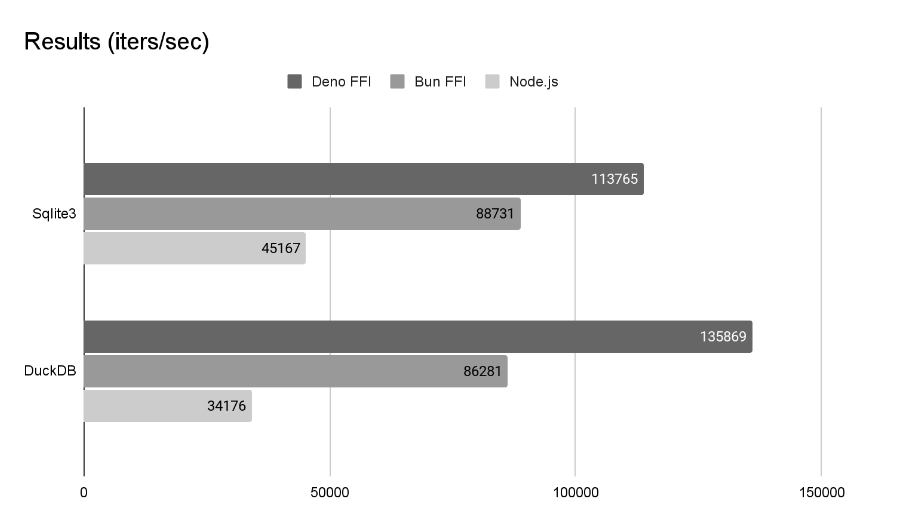
\includegraphics[width=0.38\textwidth]{assets/deno.png}
\end{center}
\caption{Benchmark comparing Deno, Bun and Node.js on Sqlite and DuckDB}
\end{wrapfigure}

This is running sqlite3 and duckdb benchmarks on Deno, Bun and Node.js. See benchmark source. \footnote{\url{https://github.com/littledivy/blazing-fast-ffi-talk}}

\section{Turbocall in action}

Slide from the DenoFest talk:

\begin{wrapfigure}{l}{0.4\textwidth}
\begin{center}
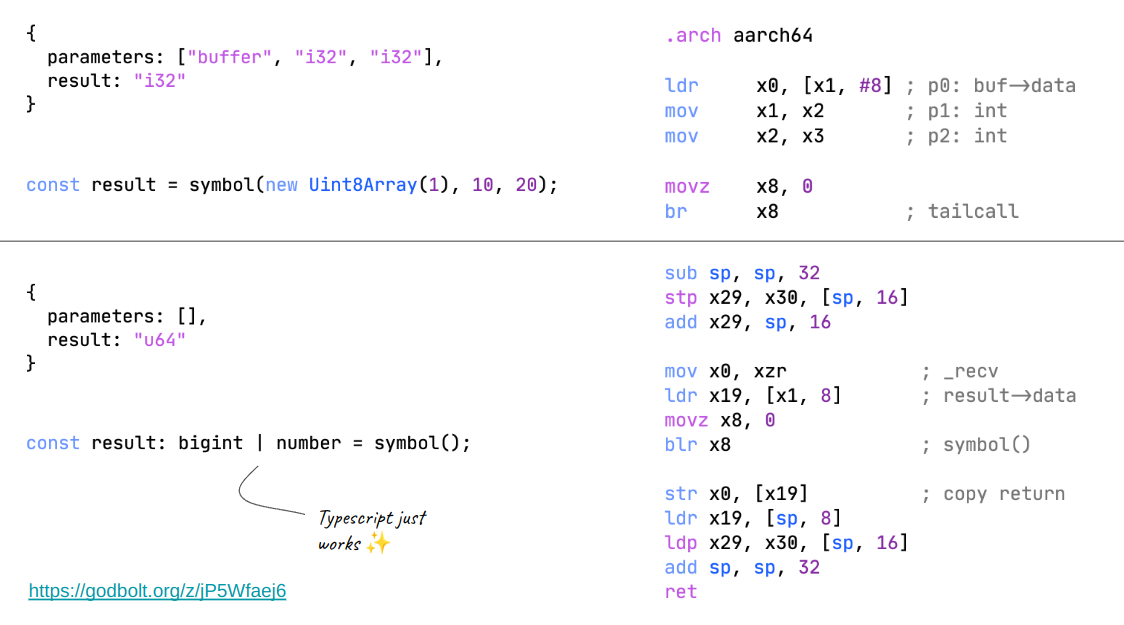
\includegraphics[width=0.38\textwidth]{assets/turbocall-slide.png}
\end{center}
\caption{Turbocall slide}
\end{wrapfigure}

\section{Future}

It will be interesting to see how Static Hermes\footnote{\url{https://tmikov.blogspot.com/2023/09/how-to-speed-up-micro-benchmark-300x.html}} will compare against 
V8 fast calls. Both can probably generate similar code at runtime but implemented very differently.

I'm also excited about `just-js/lo`\footnote{\url{https://github.com/just-js/lo}} which is a WIP low-level JS runtime that 
aims to generate V8 fast calls bindings ahead-of-time (similar to Deno) but also allow for
a more engine-agnostic design where you could swap out V8 for other engines like Hermes, Quickjs.

That's it! Feel free to follow me on Twitter: \url{https://twitter.com/undefined_void}

This document is available as PDF: \url{https://divy.work/pdf/turbocall.pdf}

\end{document}
